\documentclass[handout]{beamer}
\everymath{\displaystyle}
\mode<presentation>
{\usetheme{Warsaw}\setbeamercovered{dynamic}}
\usecolortheme{crane}
\usepackage{beamerfoils}
\pgfdeclareimage[height=1in]{university-logo}{ISULogo}
\logo{\pgfuseimage{university-logo}}
\setbeamertemplate{navigation symbols}{}
\title[\S2]{Section 2\\Theoretical probability}
\author{Dr Marcus Bishop}
\subject{Math 104}
\beamerdefaultoverlayspecification{<+->}
\theoremstyle{definition}
\newtheorem{remark}{Remark}
\newtheorem{impact}{Impact}
\newtheorem{notation}{Notation}
\begin{document}
\begin{frame}\titlepage\end{frame}
\LogoOff

\begin{frame}{Equally likely outcomes}
\begin{definition} If each outcome of experiment
as likely to occur as any other, outcomes called
\alert{equally likely}
\end{definition}
\begin{example}
Outcomes $1,2,3,4,5,6$ of rolling die equally likely
\end{example}
\begin{example}
Outcomes H,T of flipping coin equally likely
\end{example}
\begin{example}
\begin{itemize}
\item Experiment: roll two dice and add results
\item Outcomes 2,3,\ldots,12 \alert{not} equally likely!
\end{itemize}
\end{example}
\end{frame}

\begin{frame}{Example}
\begin{itemize}
\item All possible outcomes of rolling two dice:
\[\begin{array}{llllll}
\left(1,1\right)&
\left(1,2\right)&
\left(1,3\right)&
\left(1,4\right)&
\left(1,5\right)&
\alert{\left(1,6\right)}\\
\left(2,1\right)&
\left(2,2\right)&
\left(2,3\right)&
\left(2,4\right)&
\alert{\left(2,5\right)}&
\left(2,6\right)\\
\left(3,1\right)&
\left(3,2\right)&
\left(3,3\right)&
\alert{\left(3,4\right)}&
\left(3,5\right)&
\left(3,6\right)\\
\left(4,1\right)&
\left(4,2\right)&
\alert{\left(4,3\right)}&
\left(4,4\right)&
\left(4,5\right)&
\left(4,6\right)\\
\left(5,1\right)&
\alert{\left(5,2\right)}&
\left(5,3\right)&
\left(5,4\right)&
\left(5,5\right)&
\left(5,6\right)\\
\alert{\left(6,1\right)}&
\left(6,2\right)&
\left(6,3\right)&
\left(6,4\right)&
\left(6,5\right)&
\left(6,6\right)
\end{array}\]
\item Each outcome equally likely
\item Outcomes with sum $7$ shown in \alert{red}
\item Six ways to get sum $7$
\item In contrast only \alert{one} way to get sum $2$, namely $\left(1,1\right)$
\item So outcome much more likely to be $7$ than $2$
\item[]
\begin{tabular}{c|c}
{\bf Experiment}&{\bf Outcomes equally likely}\\\hline
Rolling two dice&Yes\\\hline
Rolling two dice and adding&No
\end{tabular}
\end{itemize}
\end{frame}

\begin{frame}{Theoretical probability}
\begin{definition} The \alert{[theoretical] probability} $P\left(E\right)$
of event $E$ given by
\[P\left(E\right)
=\frac{\text{Number of outcomes in $E$}}{\text{Number of possible outcomes}}\]
\end{definition}
\begin{example}
\begin{itemize}
\item Experiment: roll a die
\item $E$: Die shows $5$
\item $P\left(E\right)=\frac{1}{6}$ since six outcomes possible,
only one of which $5$
\end{itemize}
\end{example}
\begin{example}
\begin{itemize}
\item Experiment: flip a coin
\item $E$: Die shows heads
\item $P\left(E\right)=\frac{1}{2}$ since two outcomes possible,
only one of which heads
\end{itemize}
\end{example}
\end{frame}

\begin{frame}{Example}
\begin{itemize}
\item Experiment: roll two dice and add results
\item $E$: Sum is $2$
\item So $E=\left\{\left(1,1\right)\right\}$
\item $P\left(E\right)=\frac{1}{36}$
\item $F$: Sum is $7$
\item So $F=\left\{\left(1,6\right),
\left(2,5\right),\left(3,4\right),
\left(4,3\right),\left(5,2\right),\left(6,1\right)\right\}$
\item $P\left(F\right)=\frac{6}{36}=\frac{1}{6}$
\end{itemize}
\begin{remark}
\begin{itemize}
\item Finding the total number of outcomes, number of outcomes in $E$
generally involves \alert{listing} all the outcomes
\item Can be tedious
\item Would be more convenient to avoid listing outcomes, see \S5, \S6, \S8,
\S9, \S10, \S11
\end{itemize}
\end{remark}
\end{frame}

\begin{frame}{Playing cards}
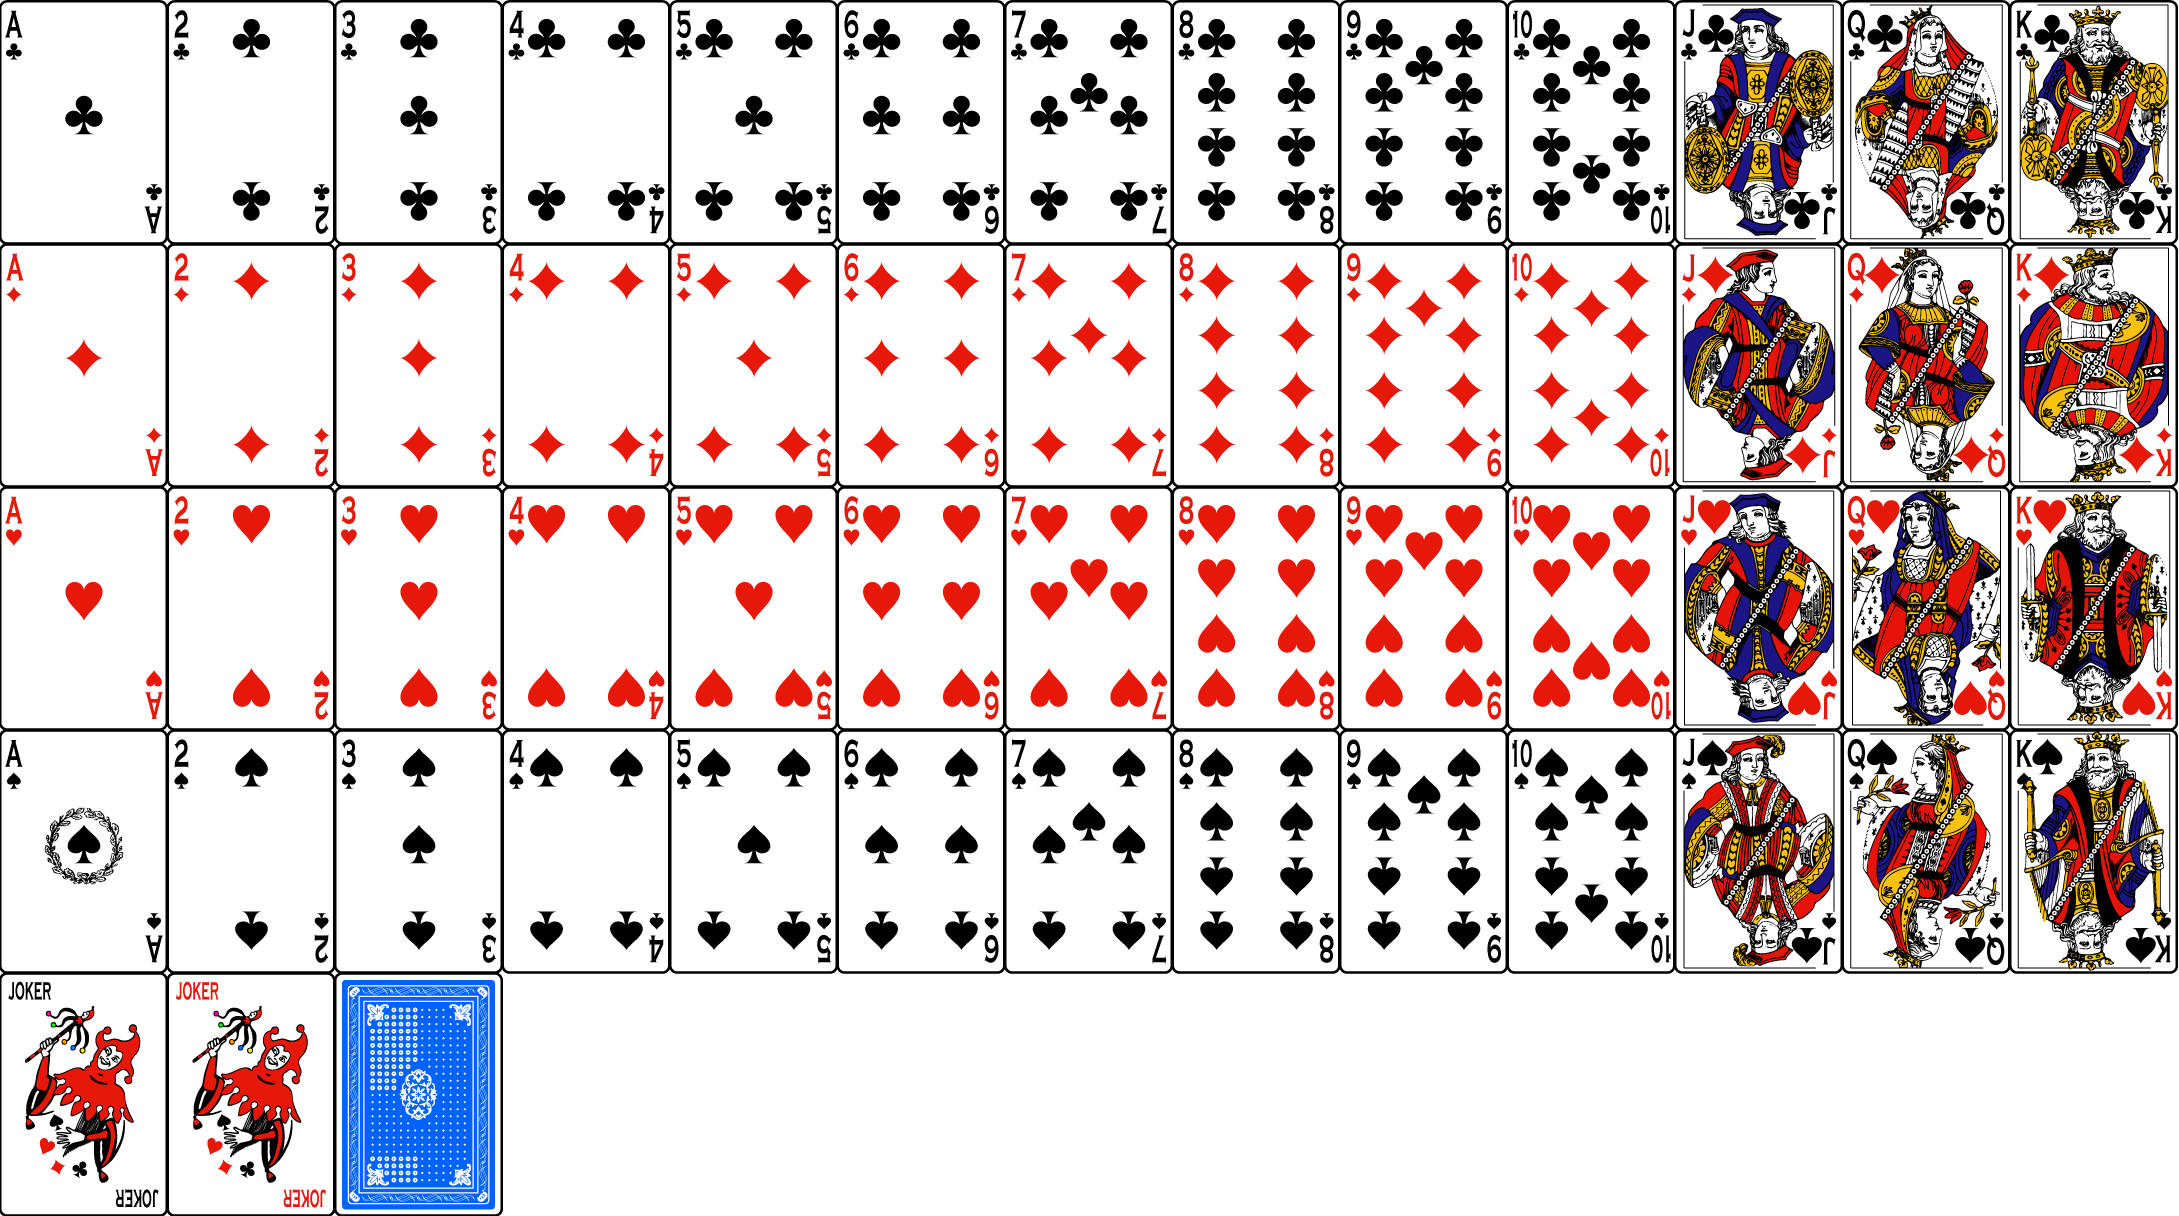
\includegraphics[scale=.15]{cards}
\begin{itemize}
\item Suits: $\spadesuit,\diamondsuit,\heartsuit,\spadesuit$
\item Colors: red, black
\item Values: $A,2,3,4,5,6,7,8,9,10,J,Q,K$
\end{itemize}
\end{frame}

\begin{frame}{Card Examples}
\begin{itemize}
\item Randomly selected card chosen
\item Calculate\dots
\item $P\left\{4\right\}\only<+->{=\frac{4}{52}}
\only<+->{=\frac{1}{13}}
\only<+->{=P\left\{5\right\}=P\left\{\text{Jack}\right\}=\cdots}$
\item $P\left\{\text{not $4$}\right\}\only<+->{=\frac{48}{52}}$
\item $P\left\{\heartsuit\right\}
\only<+->{=\frac{13}{52}}\only<+->{=\frac{1}{13}}
\only<+->{=P\left\{\spadesuit\right\}
=P\left\{\diamondsuit\right\}
=P\left\{\clubsuit\right\}}$

\end{itemize}
\end{frame}

\end{document}
